% 	This template is  MIT licensed.

% 	Basic file to demonstrate the usage of this LaTeX template.
% 	You can build your own paper/thesis on top of this file.
% 	Simply adjust the document class and all metadata and start working.
%
\documentclass[
	language=english, % set to english or german
	type=master, % set to bachelor, master or seminar
]{isthesis}

\usepackage[utf8]{vietnam}

% custom package
\usepackage{eurosym}
\usepackage{makecell}
\usepackage{hyperref}
\usepackage[utf8]{inputenc}
\usepackage{tabto} 

% Graphics rendering using TikZ
% See: https://en.wikibooks.org/wiki/LaTeX/PGF/TikZ
\usepackage{tikz}
% Include required TikZ libraries here, some exemplary libraries are pre-included
\usetikzlibrary{calc}
\usetikzlibrary{matrix}
\usetikzlibrary{positioning}
\usetikzlibrary{shapes.geometric}

%Add your library here
\addbibresource{library.bib}

% Import acronyms
% \newacronym[longplural={<long plural>}, shortplural={<short plural>}]{<label>}{<short>}{<long>}
% 	label = is the unique identifier and sort key for the acronym, can be the same as <short>
%	short = is the abbreviation or acronym
%	short plural (optional) = is the plural of the abbreviation or acronym
%	long = is the long form of the acronym, this will appear in the list of abbreviations
%	long plural (optional) = is the long plural form of the abbreviation or acronym

\newacronym[shortplural={KMUen}, longplural={Kleine und Mittlere Unternehmen}]{kmu}{KMU}{Kleines und Mittleres Unternehmen}
\newacronym{CD}{CD}{Corporate Design}
\newacronym{SQL}{SQL}{Structured Query Language}
\newacronym{FAU}{FAU}{Khoa Toán cơ tin}
\newacronym{BPM}{BPM}{Business Process Management}
\newacronym{npm}{NPM}{Node Package Manager}
\newacronym{diss}{DISS}{Digital Industrial Service System}

% Import symbols
% Syntax: <Symbol> <Label> <Name>
% The symbols are sorted by their labels
\addsymboltolist{$\Pi$}{Pi}{Projection}
\addsymboltolist{$\Join$}{Join}{Natural Join}
\addsymboltolist{$\sigma$}{Selection}{Selection}


% Import custom commands
% If you want to define custom commands, please do so here

% Import custom code block
% define listing code
\definecolor{codegreen}{rgb}{0,0.6,0}
\definecolor{codegray}{rgb}{0.5,0.5,0.5}
\definecolor{codepurple}{rgb}{0.58,0,0.82}
\definecolor{backcolour}{rgb}{0.95,0.95,0.92}

\lstdefinestyle{mystyle}{
    backgroundcolor=\color{backcolour},   
    commentstyle=\color{codegreen},
    keywordstyle=\color{magenta},
    numberstyle=\tiny\color{codegray},
    stringstyle=\color{codepurple},
    basicstyle=\ttfamily\footnotesize,
    breakatwhitespace=false,         
    breaklines=true,                 
    captionpos=b,                    
    keepspaces=true,                 
    numbers=left,
    firstnumber=1,
    stepnumber=1,                    
    numbersep=5pt,                  
    showspaces=false,                
    showstringspaces=false,
    showtabs=false,                  
    tabsize=2,
    framesep=10pt,
    xleftmargin=10pt,
    xrightmargin=10pt,
    framexleftmargin=16pt,
    framextopmargin=2pt,
    framexbottommargin=2pt, 
    frame=tb, framerule=0pt,
}

\lstset{style=mystyle}

% Document meta information
\isthesis{
    title={TIỂU LUẬN},
    sub-title={Khai phá dữ liệu và học máy \\
    Tấn công Elastic-Net vào mạng thần kinh sâu \\ 
    qua một số  mẫu đối nghịch},
    author-name={Nguyễn Mạnh Linh, Đào Thị Thu Hồng}, 
    % Separate multiple authors with commas
    % author-email={linhnguyen.code@gmail.com},
    % author-matriculation={MATRICULATION NUMBER},
    % author-phone={+49 XXXXXXXXX}, % Use international numbers format
    % author-address={STREET},
    % author-zip={ZIP},
    % author-city={CITY},
    principal-supervisor={Trần Trọng Hiếu}, % This must be a professor
    % associate-supervisor={SUPERVISOR}, % This is your main supervisor, i.e., a post doc or doctoral student
    tutor-supervisor={}, % If required, define an additional supervisor resp. tutor here
    group-institute={Đại học Khoa học Tự nhiên},
    % group={Image Data Exploration and Analysis (IDEA) Lab},
    % studies={M.Sc. International Information Systems}, %your field of studies, i.e. Wirtschaftsinformatik or International Information Systems
    %
    %associate-group={}, % When the thesis is done in cooperation with another chair, add it here
    %associate-group-institute={}, % add cooperating institute or university here
    seminar={SEMINAR}, % The title of your seminar
    submission-date={2022-10-01}, % The date you handed in your document: Format yyyy-mm-dd
    primary-logo={assets/hus.png}, % Uses the FAU logo by default
    %primary-logo-height={}, % Uses 16mm as default height
    %secondary-logo={}, % Logo of the secondary institution (cooperating chair/university), USES Faculty logo by default
    %secondary-logo-height={} % Uses 16mm as default height
}


\begin{document}
    % Title page
    \newcounter{savepage}
    \maketitle

	% Quote
    % You can put an optional quote page in front of your content
    %   \quotepage[author={Arthur C. Clarke}]{
    %   	        Any sufficiently advanced technology is indistinguishable from magic.
    %   }
    
    % Table of contents
    \tableofcontents

    \begin{abstract}
    Các nghiên cứu gần đấy đã chỉ ra tính dễ bị tổn thương của các mạng nơ ron sâu 
    (Deep Neural Networks - DNNs) đến các mẫu đối thủ - một cách trực quan, hình ảnh
    đối thủ không thể phân biệt có thể được tạo ra một cách dễ dàng khiến các mô hình 
    được huấn luyện tốt cũng phân loại ảnh sai. Các phương pháp hiện có để tạo ra mẫu 
    đối thủ thường dựa trên thông số biến dạng $L_2$ và $L_{\infty}$. Mặc dù trong 
    thực tế độ biến dạng $L_1$ là quan trọng và quyết định đến tính thưa của nhiễu lại 
    ít được xem xét. \\
    Trong bài này, chúng tôi thiết kế một quy trình tấn công DNNs thông qua mẫu đối thủ
    như một bài toán tối ưu hóa sử dụng hiệu chỉnh elastic-net. Tấn công DNNs bằng 
    elastic-net (EAD) với tham số $L_1$ được thêm vào cùng với tấn công $L_2$. 
    Kết quả thực nghiệm trên các tập dữ liệu MNIST, CIFAR10 và ImageNet chỉ ra rằng
    EAD có thể mang lại một tập mẫu đối thủ với độ nhiều $L_1$ nhỏ và đạt được hiệu 
    suất tấn công tương đương với các phương pháp hiện đại nhất qua các kịch bản tấn 
    công khác nhau. Quan trọng hơn, EAD dẫn đến sự cải tiến trong việc tấn công DNN và
    gợi ý những hiểu biết mới về hiệu chỉnh $L_1$ để cải thiện bảo mật trong các mô 
    hình học máy.
\end{abstract} 

    % \begin{abstract}
	%     % Add your abstract here:
        
	% 	% \lipsum[1]
	% \end{abstract}

    % List of figures (if you have figures)
    % \listoffigures

    % List of tables (if you have tables)
    % \listoftables
    
    % List of listings (if you have listings)
	% \lstlistoflistings

    % List of abbreviations (if you use acronyms)
    %\listofabbreviations

    % List of symbols (if you use symbols)
    %\listofsymbols
	
	% Abstract
	%
	% Comment out this part, if you don't require an abstract

	
	% storing the last pagenumber
    \setcounter{savepage}{\value{page}}
    
    
    % Content
    \begin{content}
        % Add your content files:
        \chapter{Giới thiệu}
Mạng nơ ron sâu (DNNs) 

        \chapter{Các nghiên cứu liên quan}
Trong phần này, chúng tôi tổng hợp các nghiên cứu liên quan về tấn công và phòng thủ DNNs.

\section{Tấn công vào DNNs}
\underline{FGM và I-FGM:} Kí hiệu $\mathbf{x_0}$ và $\mathbf{x}$ lần lượt là mẫu gốc và mẫu đối thủ,
$t$ là lớp mục tiêu cần tấn công. Các phương pháp đạo hàm nhanh (\textit{fast gradient 
methods - FGM}) sử dụng gradient $\nabla J$ của hàm mất mát trong tập huấn luyện $J$ với $\mathbf{x_0}$
để tạo ra các mẫu đối thủ (Goodfellow, Shlens, and Szegedy 2015). Với tấn công $L_{\infty}$, 
$\mathbf{x}$ được tính bằng công thức:
\begin{equation}
    \mathbf{x} = \mathbf{x_0} - \epsilon \times \text{sign}(\nabla J(\mathbf{x_0}, t))
\end{equation}
Trong đó $\epsilon$ là độ biến dạng $L_{\infty}$ giữa $\mathbf{x}$ và $\mathbf{x_0}$ và 
$\text{sign}(\nabla J)$ là dấu của gradient. Với tấn công $L_1$ và $L_2$, $\mathbf{x}$ 
được tính bằng công thức:
\begin{equation}
    \mathbf{x} = \mathbf{x_0} - \epsilon \frac{\nabla J(\mathbf{x_0}, t)}
    {\lVert \nabla J(\mathbf{x_0}, t) \rVert _q}
\end{equation}
với $q = 1,2$ và $\epsilon$ là độ méo tương quan. Các phương pháp lặp đạo hàm nhanh 
(\textit{Iterative fast gradient methods (I-FGM)}) được trình bày trong (Kurakin, Goodfellow, 
and Bengio 2016b) là phương pháp lặp sửa dụng FGM với một độ méo mịn hơn. Các cuộc tấn công 
không mục tiêu sử dụng FGM và I-FGM có thể được thực hiện theo cách tương tự nhau. \\

\underline{C\&W attack:} Thay vì sử dụng hàm mất mát trên tập huấn luyện Carlini và Wagner
đã thiết kế  một hiệu chỉnh $L_2$ trong hàm mất mát dựa trên lớp logit trong DNNs để sinh 
ra các mẫu đối thủ (Carlini and Wagner 2017b). Công thức này hóa ra là một trường hợp riêng của 
thuật toát EAD của chúng tôi (sẽ được trình bày trong phần sau). Tấn công C\&W được coi 
là một trong những tấn công mạnh nhất đối với DNNs vì nó có thể phá vỡ cả những DNNs được 
phòng thủ và chắt lọc, nó cũng có thể đạt được hiệu suất đáng kể với tấn công chuyển giao. \\

\underline{DeepFool:} là một thuật toán tân công không mục tiêu $L_2$ (Moosavi-Dezfooli, 
Fawzi, and Frossard 2016) dựa trên lý thuyết về phép chiếu tới siêu phẳng phân tách gần nhất
trong phân lớp. Nó cũng được sử dụng để tạo ra một nhiễu loạn phổ quát nhằm đánh lừa 
các DNN được huấn luyện trên các hình ảnh tự nhiên (Moosavi-Dezfooli et al. 2016).

\section{Phòng thủ trong DNNs}
\underline{Defensive distillation:} Chưng cất phòng thủ (Papernot et al.2016b) bảo vệ 
chống lại sự nhiễu loạn của đối thủ bằng cách sử dụng kỹ thuật chưng cất trong (Hinton, 
Vinyals, and Dean 2015) để huấn luyện lại cùng một mạng với xác suất lớp được dự đoán bởi 
mạng ban đầu. Phương pháp này đưa ra tham số nhiệt độ $T$ trong lớp softmax để tăng cường 
độ mạnh đối với những xáo trộn của mẫu đối thủ.

		\chapter{EAD: Tấn công Elastic-Net vào mạng DNNs}
\section{Sơ bộ về hiệu chỉnh Elastic-Net}
Hiệu chỉnh elastic-net là công nghệ được sử dụng rộng rãi trong việc giải quyết 
các bài toán lựa chọn thuộc tính nhiều chiều (Zou and Hastie 2005). Nó được xem 
là công cụ hiệu chỉnh trong đó tổ hợp tuyến tính hàm phạt (\textit{penalty})
$L_1$ và $L_2$. Nhìn chung, hiệu chỉnh elastic-net được sử dụng trong bài toán cực 
tiểu hóa sau đây:
\begin{equation}
    \label{eq:3.1}
    \text{minimize}_{\mathbf{z} \in \mathcal{Z}} \text{ }
    f(\mathbf{z}) + \lambda_1 \lVert \mathbf{z} \rVert_1
    + \lambda_2 \lVert \mathbf{z} \rVert_2^2
\end{equation}
Trong đó $\mathbf{z}$ là vector của $p$ biến tối ưu, $\mathcal{Z}$ là tập nghiệm 
chấp nhận được, $f(\mathbf{z})$ là hàm mất mát, $\lVert \mathbf{z} \rVert_q$ là 
chuẩn $q$ của $\mathbf{z}$ và $\lambda_1, \lambda_2 \geq 0$ tương ứng là các tham số hiệu 
chỉnh $L_1$ và $L_2$. Biểu thức $\lambda_1 \lVert \mathbf{z} \rVert_1 + \lambda_2 
\lVert \mathbf{z} \rVert_2^2$ là được gọi là hiệu chỉnh elactic-net của $\mathbf{z}$.
Với bài toán hồi quy chuẩn, hàm mất mát $f(\mathbf{z})$ là hàm lỗi trung trung bình
bình phương (\textit{mean squared error - MSE}), vector $\mathbf{z}$ biểu diễn trọng 
số của các thuộc tính và $\mathcal{Z} = \mathbb{R}^p$. Hiệu chỉnh elastic-net trong 
phương trình \ref{eq:3.1} chính là công thức Lasso khi $\lambda_2 = 0$ và trở thành công 
thức hồi quy Ridge khi $\lambda_1 = 0$. (Zou and Hastie 2005) đã chỉ ra rằng hiệu chỉnh 
elastic-net có thể chọn ra 1 nhóm các thuộc tính tương quan mạnh, mà có thể khắc phục sự 
thiếu sót của việc chọn lựa thuộc tính nhiều chiều khi sử dụng 1 mình hồi quy Lasso 
hoặc Ridge.
\section{Xây dựng thuật toán EAD}

Từ tấn công C\&W (Carlini and Wagner 2017b), ta thêm vào cùng hàm mất mát $f$ để sinh 
ra các mẫu đối nghịch. Đặc biệt, cho trước 1 ảnh $\mathbf{x_0}$ và nhãn đúng của nó là $t_0$, 
gọi $\mathbf{x}$ là mẫu đối nghịch của $\mathbf{x_0}$ với lớp đích nhắm đến là $t \neq t_0$ . Hàm mất mát 
$f(\mathbf{x})$ cho tấn công nhắm đích là:
\begin{equation}
    \label{eq:3.2}
    f(\mathbf{x}, t) = \max { \left( \max_{j \neq t} [\textbf{Logit}(\mathbf{x})]_j - 
    [\textbf{Logit}(\mathbf{x})]_t, -\kappa \right) }
\end{equation}
Trong đó $\textbf{Logit}(\mathbf{x}) = [\textbf{Logit}(\mathbf{x})_1, ..., 
\textbf{Logit}(\mathbf{x})_K] 
\in \mathbb{R}^K$ là lớp logit (lớp trước softmax) biểu diễn cho $\mathbf{x}$ trong mạng DNN, $K$
là số lượng lớp cần phân loại, $\kappa > 0$ là tham số tin cậy, nó đảm bảo một khoảng 
cách cố định giữa $\max_{j \neq t} [\textbf{Logit}(\mathbf{x})]_j$ và $[\textbf{Logit}(\mathbf{x})]_t$. 

Cần lưu ý rằng, thành phần $[\textbf{Logit}(x)]_t$ là xác xuất dự đoán $x$ có nhãn $t$ theo 
luật phân loại của hàm softmax:
\begin{equation}
    \label{eq:3.3}
    \text{Prob}(\text{Label}(\mathbf{x}) = t) = \frac{\exp([\textbf{Logit}(\mathbf{x})]_t)}{
        \sum_{j=1}^{K} \exp([\textbf{Logit}(\mathbf{x})]_j)
    }
\end{equation}
Do đó, hàm mất mát trong phương trình \ref{eq:3.2} có mục đích là để cho ra nhãn $t$ là 
lớp có xác xuất cao nhất của $x$ và tham số $\kappa$ đảm bảo sự phân biệt giữa lớp $t$
và lớp dự đoán gần nhất khác với $t$. Với tấn công không nhắm mục tiêu, hàm mất mát trong 
phương trình \ref{eq:3.2} trở thành:
\begin{equation}
    \label{eq:3.4}\
    f(\mathbf{x}) = \max { \left([\textbf{Logit}(\mathbf{x})]_{t_0} - 
    \max_{j \neq t} [\textbf{Logit}(\mathbf{x})]_j, -\kappa \right) }
\end{equation}
Trong bài viết này, chúng tôi tập trung vào tấn công nhắm mục tiêu vì nó khó hơn là không 
nhắm mục tiêu. Thuật toán EAD có thể được áp dụng trực tiếp vào tấn công không nhắm mục 
tiêu bằng cách thay $f(\mathbf{x},t)$ trong phương trình \ref{eq:3.2} thành $f(\mathbf{x})$ trong phương 
trình \ref{eq:3.4}. 

Ngoài ra, để thao túng kết quả dự đoán thông qua hàm mất mát trong \ref{eq:3.2}, hiệu chỉnh 
elastic-net còn tạo ra mẫu đối nghịch tương tự với ảnh gốc. Công thức tấn công elastic-net
vào mạng DNNs (EAD) để tạo ra mẫu đối nghịch $(\mathbf{x},t)$ cho ảnh gốc $(\mathbf{x_0}, t_0)$ như sau:
\begin{equation}
    \label{eq:3.5}
    \begin{split}
    &\text{minimize}_{\mathbf{x}} \text{ }
    c \times f(\mathbf{x}, t) + \beta \lVert \mathbf{x} - \mathbf{x_0} \rVert_1
    + \lVert \mathbf{x} - \mathbf{x_0} \rVert_2^2 \\
    &\text{st   } \mathbf{x} \in [0,1]^p
    \end{split}
\end{equation}
Với $f(\mathbf{x},t)$ được xác định trong phương trình \ref{eq:3.2}, $c, \beta \geq 0$ lần lượt 
là các tham số  hiệu chỉnh của hàm mất mát $f$ và hàm phạt $L_1$. Miền ràng buộc 
$\mathbf{x} \in [0,1]^p$ giữ cho $\mathbf{x}$ trong một không gian ảnh mà có thể dễ dàng thỏa mãn điều kiện
bằng cách chia mỗi giá trị của pixel cho giá trị lớn nhất (ví dụ $255$). Để xác định Khoảng 
cách (nhiễu) giữa $\mathbf{x}$ và $\mathbf{x_0}$ bằng $\mathbf{\delta} = \mathbf{x} - \mathbf{x_0}$,
công thức EAD trong \ref{eq:3.5} được tạo ra để tìm một mẫu đối nghịch $\mathbf{x}$ mà sẽ 
được phân loại vào lớp mục tiêu $t$, đồng thời cực tiểu hóa $\mathbf{\delta}$ trong hàm
mất mát elastic-net $\beta \lVert \mathbf{\delta} \rVert_1 + \lVert \mathbf{\delta} \rVert_2^2$.
Đáng chú ý, công thức tấn công C\&W (Carlini and Wagner 2017b) trở thành trường hợp đặc biệt 
của EAD trong công thức \ref{eq:3.5} khi $\beta = 0$ , không phụ thuộc vào $L_1$ của $\mathbf{\delta}$.
Tuy nhiên thành phần phạt $L_1$ là một hiệu trực quan để tạo ra mẫu đối nghịch do 
$\lVert \mathbf{\delta} \rVert_1 = \sum_{i=1}^p |\mathbf{\delta_i}|$ biểu diễn tổng sai khác
của nhiễu và được sử dụng rộng rãi như là hàm thay thế để phát triển các nhiễu thưa. 
Phần đánh giá hiệu năng sẽ chứng minh rằng khi đưa thành phần $L_1$ vào nhiễu sẽ sinh ra 
tập phân biệt các mẫu đối nghịch, và nó cải thiện khả năng chuyển giao tấn công và triển 
khai huấn luyện đối nghịch.


        \chapter{Đánh giá hiệu năng}
Trong phần này, chúng ta so sánh EAD với các thuật toán tấn công tiên tiến hiện nay trên 3 
tập dữ liệu ảnh: MNIST, CIFAIR10 và ImageNet. Tác giả bài viết muốn cho thấy:
\begin{itemize}
    \item EAD có thể thu được hiệu năng tấn công tương tự tấn công C\&W đối với mạng DNN 
    phòng thủ và mạng DNN không phòng thủ do C\&W là trường hợp đặc biệt của EAD khi 
    $\beta = 0$.
    \item So sánh với các phương pháp tấn công hiện tại dựa trên $L_1$ như FGM, I-FGM, 
    các mẫu đối nghịch thu được từ EAD có nhiễu $L_1$ nhỏ hơn đáng kể và tỷ lệ tấn công 
    thành công cao hơn.
    \item Các mẫu đối nghịch tạo bởi EAD có thể hỗ trợ chuyển giao tấn công và triển khai 
    huấn luyện đối nghịch.
\end{itemize}
\section{Các phương pháp đối sánh}
Bài viết này so sánh EAD với các phương pháp tấn công nhắm đích hiệu quả nhất có sử dụng 
các loại hiệu chỉnh khác nhau:
\begin{itemize}
    \item C\&W: tấn công nhắm đích dùng hiệu chỉnh $L_2$ được đề xuất bởi Carlini and agner (Carlini and Wagner 2017b). Đây là trường hợp đặc biệt của EAD khi $\beta = 0$.
    \item FGM (fast gradient method): được đề xuất bởi (Goodfellow, Shlens, and Szegedy 2015). FGM sử dụng nhiều loại hiệu chỉnh với các phiên bản FGM-$L1$, FGM-$L_1$, FGM-$L_{\infty}$.
    \item I-FGM: (FGM lặp): được đề xuất bởi (Kurakin, Goodfellow, and Bengio 2016b). I-FGM sử dụng nhiều loại hiệu chỉnh I-FGM-$L_1$, I-FGM-$L_2$, I-FGM-$L_{\infty}$.
\end{itemize}
\section{Thiết kế thực nghiệm}
Thực nghiệm sử dụng framework của Carlini và Wagner. Với cả tấn công EAD và C\&W, tác giả đều sử dụng các tham số cấu hình mặc định, trong đó triển khai 9 bước tìm kiếm nhị phân trên tham số hiệu chỉnh  (bắt đầu từ 0.001) và chạy  vòng lặp cho mỗi bước với learning rate khởi tạo . Để tìm các mẫu đối nghịch thành công, tác giả sử dụng thuật toán tối ưu tham chiếu (ADAM) cho C\&W, và sử dụng thuật toán chiếu FISTA (thuật toán 1) với square-root decaying learning rate cho EAD. Tương tự tấn công C\&W, mẫu đối nghịch cuối cùng tìm được từ EAD được chọn là mẫu nhiễu ít nhất giữa các mẫu đối nghịch thành công. Độ nhạy cảm của L1 (tham số  ) và tác động của luật chọn trong EAD sẽ được bàn đến ở phần sau. Tác giả đặt tham số tấn công chuyển giao $\kappa = 0$ cho cả EAD và C\&W.
\begin{center}
    \resizebox{\textwidth}{!}{
    \begin{tabular}{cc|c|c|c}
        \hline
        && Best case & Average case & Worst case \\
        \hline
        Optimization method & $\beta$  
        & \begin{tabular}{cccc}
            ASR & $L_1$ & $L_2$ & $L_{\infty}$
        \end{tabular}
        & \begin{tabular}{cccc}
            ASR & $L_1$ & $L_2$ & $L_{\infty}$
        \end{tabular}
        & \begin{tabular}{cccc}
            ASR & $L_1$ & $L_2$ & $L_{\infty}$
        \end{tabular} \\  
        \hline    
    \end{tabular}}
\end{center}

Tác giả triển khai FGM và I-FGM bằng gói thư viện CleverHans. Tham số nhiễu tốt nhất $\epsilon$ được xác định bằng phương pháp tìm kiếm lưới fine-grained trên mỗi ảnh, $\epsilon$ nhỏ nhất trong lưới thể hiện tấn công thành công sẽ được ghi lại. Với I-FGM, tác giả thực hiện $10$ vòng lặp FGM ($10$ là giá trị mặc định) với $\epsilon$-ball clipping. Tham số nhiễu $\epsilon'$ trong mỗi vòng lặp FGM được đặt là $\epsilon/10$ , đã được chứng minh hiệu quả trong (Tram`er et al. 2017). Dải giá trị của lưới và độ phân giải của 2 phương pháp trên được đề cập cụ thể trong tài liệu bổ sung 1.

Việc phân loại ảnh cho tập MNIST và CIFAIR10 được huấn luyện trên mô hình DNN bởi Carlini and Wagner. Để phân loại cho tập ImageNet, người ta dùng mô hình Inception-v3 (Szegedy et al. 2016). Đối với tập MNIST và CIFAIR10, tác giả lấy ngẫu nhiên trong tập test 1000 ảnh đã được phân loại đúng để tấn công làm phân loại sai. Với tập ImageNet, tác giả chọn ngẫu nhiên 100 ảnh đã được phân loại đúng và 9 ảnh được phân loại sai để tấn công. Tất cả thực nghiệm được triển khai trên thiết bị phần cứng Intel E5-2690 v3 CPU, 40 GB RAM, single NVIDIA K80 GPU.
\section{Các độ đo đánh giá}
Theo cách đánh giá trong (Carlini and Wagner 2017b), tác giải báo cáo tỷ lệ tấn công thành công và độ nhiễu của mẫu đối nghịch trong mỗi phương pháp. Tỷ lệ tấn công thành công (ASR) là phần trăm mẫu đối nghịch được phân loại vào lớp đích (khác lớp gốc). Các trung bình $L_1$, $L_2$ và $L_{\infty}$ của các mẫu đối nghịch thành công cũng được ghi chép báo cáo. Cụ thể, các trường hợp sau được quan tâm:
\begin{itemize}
    \item \textbf{Trường hợp tốt nhất (best case):} tấn công dễ nhất về phương diện nhiễu, trong số các tấn công nhắm tới tất cả các lớp sai nhãn.
    \item \textbf{Trường hợp trung bình (average case):} tấn công nhắm ngẫu nhiên vào 1 lớp sai nhãn.
    \item \textbf{Trường hợp xấu nhất (worst case):} tấn công khó nhất về phương diện nhiễu, trong số những tấn công nhắm tới tất cả các lớp sai nhãn.
\end{itemize}
\section{Phân tích độ nhạy và luật quyết định}
Tác giả kiểm tra sự cần thiết của việc sử dụng thuật toán 1 để giải bài toán tấn công bằng hiệu chỉnh elastic-net trong (\ref{eq:7}) bằng cách so sánh nó với thuật toán COV thuần. Trong tài liệu (Carlini and Wagner 2017b), Carlini và Wagner đã loại bỏ điều kiện ràng buộc $\mathbf{x} \in [0,1]^p$ bằng cách thay $\mathbf{x}$ bằng $\frac{\mathbf{1} + \tanh \mathbf{w}}{2}$ với $\mathbf{w} \in \mathbb{R}^p$ và $\mathbf{1} \in \mathbb{R}^p$ là vector các với các phần tử $1$. Thuật toán tối ưu mặc định ADAM (Kingma and Ba 2014) được sử dụng để giải ra nghiệm $\mathbf{w}$ và từ đó tìm được $\mathbf{x}$. Tác giả áp dụng thuật toán COV lên (\ref{eq:7}) và so sánh với EAD trên tập MNIST với các  khác nhau trong bảng 1 ở trên. Mặc dù COV và EAD thu được tỷ lệ tấn công thành công tương tự nhau, người ta quan sát thấy COV không hiệu quả trong việc tạo ra các mẫu đối nghịch $L_1$. Khi tăng $\beta$, EAD tạo ra ít mẫu đối nghịch $L_1$ hơn, trong khi các kết quả $L_1$, $L_2$, và $L_{\infty}$ của COV thì ít chịu ảnh hưởng khi thay đổi $\beta$. Khi sử dụng các hàm thư viện TensorFlow như AdaGrad, RMSProp, SGD, người ta cũng thấy nó ít ảnh hưởng bởi $\beta$  giống như trường hợp của COV. Nhóm tác giả cũng báo cáo rằng phương pháp COV cấm dùng ISTA vì thành phần hàm $\tanh$ trong hiệu chỉnh $L_1$. Sự ít ảnh hưởng của COV cho thấy nó không phù hợp cho tối ưu elastic-net, do nó không hiệu quả cho bài toán tối ưu bằng subgradient (Duchi and Singer 2009). Với EAD, nhóm tác giả tìm được 1 cách thú vị đánh đổi giữa $L_1$, $L_2$, và $L_{\infty}$. Điều này là do khi tăng $\beta$ làm tăng độ thưa của nhiễu và do đó tăng $L_2$, $L_{\infty}$ . Kết quả tương tự cũng được quan sát thấy với CIFAR10.
\begin{figure}[H] % places figure environment here   
    \centering % Centers Graphic
    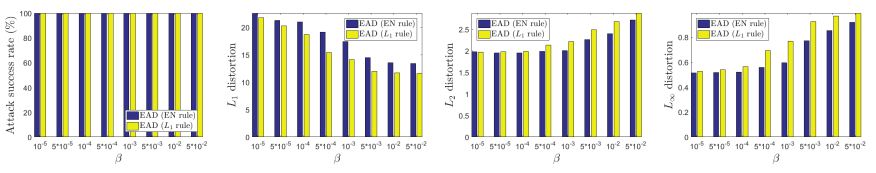
\includegraphics[width=1\textwidth]{assets/fig_02.png} 
    \caption{So sánh luật quyết định EN và $L_1$ trong EAD trên tập MNIST với nhiều tham số hiệu chỉnh $L_1$ $\beta$ (trường hợp trung bình). So sánh với luật EN cho cùng giá trị $\beta$} % Creates caption underneath graph
    \label{fig:fg_02}
\end{figure}

\begin{longtable}{l}
		\resizebox{\textwidth}{!}{
		\begin{tabular}{l|llll|llll|llll}
			\hline
			& \multicolumn{4}{c}{MNIST} & \multicolumn{4}{c}{CIFAR 10} & \multicolumn{4}{c}{ImageNet}\\
			\hline
			Attack method & ASR & $L_1$ & $L_2$ & $L_\infty$ & ASR & $L_1$ & $L_2$ & $L_\infty$ & ASR & $L_1$ & $L_2$ & $L_\infty$ \\
			\hline
			C\&W ($L_2$) & \textbf{100} & 22.46 & \textbf{1.972} & 0.514 & \textbf{100} & 13.62 & \textbf{0.392} & 0.044 & \textbf{100} & 232.2 & \textbf{0.705} & 0.03 \\
			FGM-$L_1$ & 39 & 53.5 & 4.186 & 0.782 & 48.8 & 51.97 & 1.48 & 0.152 & 1 & 61 & 0.187 & 0.007 \\
			FGM-$L_2$ & 34.6 & 39.15 & 3.284 & 0.747 & 42.8 & 39.5 & 1.157 & 0.136 & 1 & 2338 & 6.823 & 0.25 \\
			FGM-$L_\infty$ & 42.5 & 127.2 & 6.09 & 0.296 & 52.3 & 127.81 & 2.373 & 0.047 & 3 & 3655 & 7.102 & 0.014 \\
			I-FGM-$L_1$ & \textbf{100} & 32.94 & 2.606 & 0.591 & \textbf{100} & 17.53 & 0.502 & 0.055 & 77 & 526.4 & 1.609 & 0.054 \\
			I-FGM-$L_2$ & \textbf{100} & 30.32 & 2.41 & 0.561 & \textbf{100} & 17.12 & 0.489 & 0.054 & \textbf{100} & 774.1 & 2.358 & 0.086 \\
			I-FGM-$L_\infty$ & \textbf{100} & 71.39 & 3.472 & \textbf{0.227} & \textbf{100} & 33.3 & 0.68 & \textbf{0.018} & \textbf{100} & 864.2 & 2.079 & \textbf{0.01} \\
			EAD (EN rule) & \textbf{100} & \textbf{17.4} & 2.001 & 0.594 & \textbf{100} & \textbf{8.18} & 0.502 & 0.097 & \textbf{100} & \textbf{69.47} & 1.563 & 0.238 \\
			EAD ($L_1$ rule) & \textbf{100} & \textbf{14.11} & 2.211 & 0.768 & \textbf{100} & \textbf{6.066} & 0.613 & 0.17 & \textbf{100} & \textbf{40.9} & 1.598 & 0.293 \\
			\hline
		\end{tabular}} \\ 
		\caption{So sánh các tấn công trên các tập dữ liệu MNIST, CIFAR10 và ImageNet. ASR là tỷ lệ tấn công thành công (\%). Giá trị nhiễu trong bảng đo được trên giá trị trung bình của các mẫu thành công. EAD, C\&W và I-FGM-$L_\infty$ thu được các mẫu ít nhiễu nhất trên các chuẩn $L_1$,$L_2$,$L_\infty$ tương ứng. Kết quả đầy đủ được báo cáo trong tài liệu mở rộng.}
		\label{tab:tab_2}
\end{longtable}

Ở bảng \ref{tab:tab_1}, quá trình thuật toán tối ưu chạy để tìm ra mẫu đối nghịch cuối cùng giữa những mẫu đối nghịch thành công dựa trên hàm mất mát elastic-net trong $\{\mathbf{x}^{(k)}\}^I_{k=1}$, gọi là luật chọn elastic-net. Ngoài ra, có thể chọn mẫu đối nghịch cuối cùng sao cho $L_1$ nhỏ nhất, gọi là luật chọn $L_1$. Hình \ref{fig:fg_02} so sánh ASR và các nhiễu trung bình trên 2 luật chọn nói trên với các giá trị  khác nhau trên tập dữ liệu MNIST. Cả 2 luật chọn đều cho tỷ lệ thành công ASR $100\%$ với dải giá trị  rộng. Với cùng 1 giá trị , luật chọn $L_1$ cho ra các mẫu đối nghịch ít nhiễu $L_1$ hơn so với luật chọn EN, trong khi đó lại bị trả giá nhiều nhiễu hơn ở $L_2$, $L_{\infty}$ . Xu hướng tương tự cũng được quan sát thấy với CIFAR10 (kết quả đầy đủ với cả 2 tập dữ liệu MNIST và CIFAR có trong tài liệu mở rộng). Trong các thí nghiệm tiếp theo, nhóm tác giả báo cáo kết quả của EAD với 2 luật chọn và $\beta = 10^{-3}$, vì trên tập MNIST và CIFAR10 giá trị $\beta$ làm giảm nhiễu $L_1$ trong khi so sánh với $L_2$, $L_{\infty}$ với trường hợp $\beta = 0$ (nghĩa là không có hiệu chỉnh $L_1$).


\section{Tỷ lệ tấn công thành công và nhiễu trên các tập dữ liệu MNIST, CIFAR10 và ImageNet}
Nhóm tác giả so sánh EAD với các phương pháp đối sánh trên các tiêu chí tỷ lệ tấn công thành công và các nhiễu khi tấn công mạng DNN huấn luyện bởi MNIST, CIFAR10 và ImageNet. Bảng 2 là kết quả thực nghiệm. FGM ít tấn công thành công (chỉ số ASR thấp) và chỉ số nhiễu khá lớn so với các phương pháp khác. Trong khi đó, C\&W, I-FGM và EAD đều đạt ASR $100\%$. Ngoài ra, EAD, C\&W và I-FGM-$L_{\infty}$ đạt được các mẫu đối nghịch với ít nhiễu nhất lần lượt trên các chỉ số  $L_1$, $L_2$ và $L_{\infty}$. Hơn nữa, EAD tốt hơn các phương pháp $L_1$ hiện tại (ví dụ I-FGM-$L_1$). So sánh với I-FGM-$L_1$, EAD với luật chọn EN giảm nhiễu $L_1$ xuống xấp xỉ $47\%$ trên tập MNIST, $53\%$ với tập CIFAR10 và $87\%$ với ImageNet. Tác giả cũng báo cáo kết quả quan sát rằng EAD với luật chọn $L_1$ có thể giảm nhiễu $L_1$ nhưng làm tăng $L_2$ và $L_{\infty}$.



Mặc dù có nhiễu $L_2$ và $L_{\infty}$ lớn, các mẫu đối nghịch tạo bởi EAD với luật chọn $L_1$ có thể đạt ASR $100\%$ trên tất cả các tập dữ liệu. Nghĩa là nhiễu $L_2$ và $L_{\infty}$ không đủ để đánh giá sức mạnh của mạng neuron. Hơn nữa, kết quả tấn công trong bảng 2 cho thấy EAD có thể thu được 1 tập phân biệt các mẫu đối nghịch khác biệt cơ bản với các mẫu dựa trên $L_2$ và $L_{\infty}$. Tương tự phương pháp C\&W và I-FGM, các mẫu đối nghịch sinh bởi EAD đều khó phân biệt bằng mắt thường. 

\section{Phá vỡ chắt lọc phòng thủ}
Ngoài ra, để tấn công DNN không phòng thủ bằng các mẫu đối nghịch, tác giả đã cho thấy EAD có thể phá vỡ DNN chắt lọc phòng thủ. Chắt lọc phòng thủ (Papernot et al. 2016b) là kĩ thuật phòng thủ chuẩn trong đó mạng được huấn luyện lại bằng các xác suất từng lớp được dự đoán bởi một mạng gốc (chứ không phải bằng nhãn ground truth), gọi là nhãn mềm và người ta dùng tham số nhiệt $T$ trong lớp softmax để tăng cường sức mạnh của nó chống lại nhiễu đối nghịch. Tương tự như phương thức tấn công tiên tiến C\&W, hình \ref{fig:fg_03} cho thấy EAD có thể thu được ASR $100\%$ với các giá trị $T$ khác nhau trên tập MNIST và CIFAR10. Hơn nữa, vì công thức tấn công C\&W là trường hợp đặc biệt của công thức EAD trong (\ref{eq:7}) khi $\beta = 0$, sự thành công của EAD trong việc phá vỡ chắt lọc phòng thủ gợi ý 1 cách mới để tạo ra các mẫu đối nghịch hiệu quả là dùng các tham số  $\beta$ khác nhau cho hiệu chỉnh $L_1$. Kết quả đầy đủ của tấn công ở trong tài liệu mở rộng.

\begin{figure}[H] % places figure environment here   
    \centering % Centers Graphic
    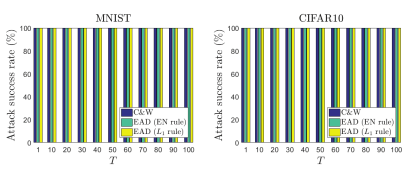
\includegraphics[width=0.8\textwidth]{assets/fig_3.png} 
    \caption{ASR (trường hợp trung bình) của C\&W và EAD trên tập MNIST và CIFAR10 với các tham số nhiệt $T$ khác nhau cho chắt lọc phòng thủ. Cả 2 phương pháp đều phá vỡ thành công chắt lọc phòng thủ.} % Creates caption  % Creates caption underneath graph
    \label{fig:fg_03}
\end{figure}
\section{Cải thiện tấn công chuyển giao}
Trong tài liệu (Carlini and Wagner 2017b) đã chỉ ra rằng tấn công C\&W có khả năng chuyển giao tốt hơn  từ 1 mạng không phòng thủ sang 1 mạng phòng thủ chưng cất bằng cách tối ưu các tham số độc lập $\kappa$ trong phương trình \ref{eq:4}. Theo (Carlini and Wagner 2017b), nhóm tác giả sử dụng cùng bộ tham số của tấn công chuyển giao trên tập MNIST, vì MNIST là tập dữ liệu khó nhất khi tấn công bằng nhiễu trung bình trên mỗi ảnh như trong bảng \ref{tab:tab_2} ở trên.

Cố định $\kappa$, các mẫu đối nghịch được sinh ra từ mạng không phòng thủ gốc được sử dụng để tấn công mạng phòng thủ chưng cất với tham số nhiệt $T = 100$ (Papernot et al. 2016b). Tỷ lệ tấn công thành công (ASR) của EAD, phương pháp C\&W và I-FGM được trình bày trong hình \ref{fig:fg_04}. Khi $\kappa = 0$, tất cả các phương pháp đều cho ASR thấp và do đó không tạo được các mẫu đối nghịch có thể chuyển giao. Tỷ lệ ASR của EAD và phương pháp C\&W cải thiện khi đặt $\kappa > 0$ , trong khi đó tỷ lệ ASR của I-FGM thấp (dưới $2\%$) do tấn công không có các tham số tương tự để có thể chuyển giao.

Chú ý rằng, EAD có thể thu được ASR gần đạt $99\%$ khi $\kappa = 50$, trong khi đó ASR cao nhất mà phương pháp C\&W đạt được là gần $88\%$ khi $\kappa = 40$. Chứng tỏ rằng, khả năng chuyển giao tấn công tăng lên khi sử dụng các mẫu đối nghịch được tạo từ EAD, điều này là do thuật toán ISTA trong phương trình \ref{eq:8} mạnh hơn so với tấn công C\&W qua phương pháp shrinking and thresholding. Nhóm tác giả cũng phát hiện rằng khi đặt $\kappa$ quá lớn cũng làm giảm ASR của các tấn công chuyển giao cả bằng EAD và phương pháp C\&W, do thuật toán tối ưu không tìm được mẫu đối nghịch có thể làm tối thiểu hóa hàm mất mát $f$ trong \ref{eq:4} khi $\kappa$ lớn. Kết quả đầy đủ của việc chuyển giao tấn công được báo cáo trong tài liệu kèm theo.

\begin{figure}[H] % places figure environment here   
    \centering % Centers Graphic
    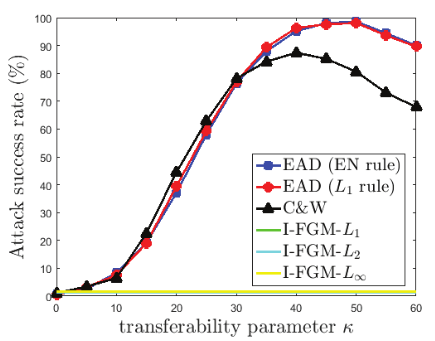
\includegraphics[width=0.5\textwidth]{assets/fig_04.png} 
    \caption{Khả năng chuyển giao tham số $\kappa$} % Creates caption  % Creates caption underneath graph
    \label{fig:fg_04}
\end{figure}
\section{Huấn luyện đối nghịch bổ sung}
Để xem xét sự khác biệt giữa các mẫu đối nghịch $L_1$ và $L_2$, tác giả kiểm tra hiệu quả huấn luyện đối nghịch trên tập MNIST. Họ chọn ngẫu nhiên $1000$ ảnh từ tập huấn luyện và sử dụng tấn công C\&W và EAD (luật chọn $L_1$) để tạo ra $9000$ mẫu đối nghịch cho tất cả các nhãn sai với mỗi phương pháp. Sau đó, họ thêm vào tập huấn luyện các mẫu đối nghịch này để huấn luyện lại mạng và kiểm tra sức mạnh của nó trên tập kiếm thử, kết quả tổng hợp trong bảng 3. Để huấn luyện đối nghịch với 1 phương pháp nào đó, mặc dù cả 2 tấn công đều đạt tỷ lệ thành công trung bình $100\%$, mạng vẫn có sức chịu đựng tốt hơn trước nhiễu đối nghịch vì các chỉ số nhiễu đều đã tăng lên đáng kể so với trường hợp chưa huấn luyện. Tác giả cũng quan sát thấy kết hợp huấn luyện bằng EAD và phương pháp C\&W có thể làm tăng hơn nữa nhiễu $L_1$ và $L_2$ so với tấn công C\&W, và tăng nhiễu $L_2$ so với EAD, với giả thiết rằng mẫu $L_1$ được tạo bởi EAD có thể được huấn luyện đối nghịch bổ sung.  

        \chapter{Kết luận}
Nhóm tác giả đã đề xuất mô hình tấn công bằng hiệu chỉnh elastic-net để tạo ra các mẫu đối nghịch trong tấn công DNN. Các kết quả thực nghiệm trên các tập dữ liệu MNIST, CIFAR10 và ImageNet cho thấy các mẫu $L_1$ tạo bởi EAD có thể đạt được tỷ lệ thành công tương đương với các phương pháp tấn công tiên tiến dựa trên $L_2$ và $L_{\infty}$ khi phá vỡ mạng không phòng thủ và phòng thủ chưng cất. Ngoài ra, EAD có thể cải thiện khả năng chuyển giao tấn công và huấn luyện đối nghịch bổ sung. Các kết quả của nhóm tác giả đã chứng minh hiệu quả của EAD và đưa ra hướng mới sử dụng mẫu đối nghịch $L_1$ trong việc huấn luyện đối nghịch và tăng cường an ninh cho DNN.
        % \chapter{Tổng quan}
Xem xét hệ phương trình tuyến tính $Ax=b$ trong đó $A \in \mathbb{C} ^{m \times m}$ 
và $b \in \mathbb{C}^m$.

Nghiệm chính xác của hệ $x_* = A^{-1}b$. Đương nhiên việc tính ma trận nghịch đảo $A^{-1}$
hoặc dùng phương pháp khử Gauss là rất tốn chi phí. Ta biết rằng độ phức tạp của thuật 
toán khi sử dụng phương pháp khủ Gauss là $O(m^3)$. Để có cái nhìn trực quan về độ phức tạp 
này, ta có thể xem qua bảng sau 

\begin{center}
    \begin{tabular}{| c | c | c |}
        \hline
        Năm & $m$ & $m^3$ \\ 
        \hline
        1950 & 20 & $2 \times 10^3$ \\
        1965 & 200 & $2 \times 10^6$ \\
        1980 & 2000 & $2 \times 10^9$ \\
        \hline
    \end{tabular}
\end{center}

Khi kích thước của ma trận tăng lên, số phép tính cũng tăng lên rất nhanh. Cùng với sự phát triển của 
phần cứng chúng ta cũng tính toán được với những ma trận với kích thước lớn hơn rất nhiều so với những
năm 1950. Nhưng ta cũng thấy rằng, khi kích thước của ma trận là hàng nghìn thì số phép tính đã là 
hàng tỉ. Với những bài toán lớn như mô phỏng thời tiết hay thiên hà trong thiên văn học, phần cứng 
máy tính không thể đuổi kịp để tính toán cũng như lưu trữ.

Điều này đòi hỏi chúng ta cần tìm ra những phương pháp tốt hơn nhằm giảm độ phức tạp của thuật toán.
Tiểu luận này giới thiệu 1 vài phương pháp với độ phức tạp $O(m^2)$.

Phương pháp lặp cho phép chúng ta tiến gần đến nghiệm chính xác của phương trình qua mỗi bước lặp.
Đến một lúc nào đó phần dư là đủ chấp nhận được, ta có nghiệm gần đúng của phương trình.

Gọi $x_n$ là nghiệm gần đúng của phương trình tại bước lặp thứ $n$. Ta định nghĩa phần dư
\begin{equation}
    r_n = b - Ax_n
\end{equation}

Khi $r_n < \epsilon$ (là một sai số nhỏ chấp nhận được) ta dừng lại và thu được nghiệm gần đúng $x_n$

Trong bài này chúng ta sẽ tìm nghiệm $x_n \in \kappa_n$, trong đó $\kappa_n$ là không gian con Krylov

\section*{Không gian con Krylov}
Cho ma trận $A \in \mathbb{C}^{m \times m}$ và vector $b \in \mathbb{C}^m$.

Dãy Krylov được định nghĩa là tập các vectors $b, Ab, A^2b, ...$.

Không gian con Krylov là không gian được sinh bởi các vectors này

Ma trận Krylov
\begin{equation}
    K_n = \begin{bmatrix}
        b & | & Ab & | & A^2b & ... & | & A^{n-1}b
    \end{bmatrix}    
\end{equation}


Trở lại bài toán, ta muốn tìm nghiệm $x_n$ trong không gian $\kappa_n$ hay nói 
các khác $x_n \in range(K_n)$. Ta có thể sử dụng phân tích $QR$ cho ma trận Krylov và
đặt $x_n = Q_ny$ trong đó $Q_n$ là ma trận unitary. 

Bài toán cực tiểu hóa $r_n$ đưa về việc cực tiểu hóa $\|AQ_ny - b\|$


Chúng ta sẽ tiếp cận bài toán với việc giải tổng quát với phương pháp GMRES 
và sử giải bài toán ma trận đối xứng như một trường hợp riêng với phương pháp MINRES.
Trước hết, thuật giải Arnoldi sẽ được giới thiệu sau đây.
        % \chapter{GMRES}
\section{Thuật giải Arnoldi}
Phương pháp GMRES sử dụng quá trình Gram-Schmitz chỉnh sửa để thiết lập
một cơ sở trực chuẩn cho không gian Krylov $span\{r_0, Ar_0, ..., A^kr_0 \}$.
Quá trình Gram-Schmitz được áp dụng cho không gian này được gọi là phương pháp \textit{Arnoldi}
Giải thuật này nhằm phân tích $A=QHQ^*$, trong đó $Q$ là ma trận trực chuẩn (unitary) 
còn $H$ là ma trận Hessenberg\footnote{
    \textit{
    Ma trận $H$ vuông kích thước $n \times n$ được gọi là ma trận upper Hessenberg nếu
    $h_{ij} = 0$ với mọi $i,j$ mà $i > j + 1$
}
}.



\textbf{Arnoldi Algorithm}
\begin{lstlisting}[style=algo]
    Given $q_1$ with $\|q_1\| = 1$
    For $j = 1, 2, ...$
        $\tilde{q}_{j + 1} = Aq_j$
        For $i = 1, ..., j$
            $h_{ij} = \langle\tilde{q}_{j+1}, q_j\rangle$
            $\tilde{q}_{j+1} \gets \tilde{q}_{j+1} - h_{ij}q_i$
        $h_{j+1,j} = \|\tilde{q}_{j+1}\|$
        $q_{j + 1} = \tilde{q}_{j+1}/h_{j+1,j}$
\end{lstlisting}


    \end{content}
    
    \pagenumbering{Roman}
    \setcounter{page}{\numexpr\value{savepage}}

    % References
    % \references{}
    
    % Appendix
    %  \begin{appendix}
    %     % In the appendices, use \section{} instead of \chapter{}
    %      \section{Some Appendix Section}
\label{sec:appendix01}
Appendices provide only two structural levels, viz., \texttt{\textbackslash section}, and \texttt{\textbackslash subsection}.

The numbering of figures, listings, tables, and footnotes is not reset. Thus, it continues as usual in the appendix.

\subsection{Some Appendix Subsection}

\lipsum[10]
    %  \end{appendix}




    % Declaration of authorship
    % \authorshipstatement[pagenumbering=false]
    % \authorshipstatement[pagenumbering=true]
    % \authorshipstatement[pagenumbering=only]
    
    % Consent form for use of plagiarism detection software
    % Not yet required
    % \consentform[pagenumbering=false]
    % \consentform[pagenumbering=true]
    % \consentform[pagenumbering=only]
    
    % Bonus: Wordcount
    % cd %FOLDER WHERE THE .tex FILES ARE IN %
    % clear
    % texcount -total -q -col -sum *.tex
    
\end{document}